\documentclass{beamer}

\mode<presentation>
{
  \usetheme{default}      % or try Darmstadt, Madrid, Warsaw, ...
  \usecolortheme{default} % or try albatross, beaver, crane, ...
  \usefonttheme{default}  % or try serif, structurebold, ...
  \setbeamertemplate{navigation symbols}{}
  \setbeamertemplate{caption}[numbered]
} 

\usepackage[utf8]{inputenc}
% \usepackage[english,greek]{babel}
\usepackage{epstopdf}
% \newcommand{\en}{\selectlanguage{english}}
% \newcommand{\el}{\selectlanguage{greek}}
\usepackage{graphicx}
\graphicspath{ {../figures/} }
\usepackage{xcolor}
\usepackage{hyperref}
\usepackage{soul} % for \st{...} aka strikethrough
\usepackage{amsmath} % for math ...
\usepackage{tikz} % drawing stuff ..
\usetikzlibrary{tikzmark,shapes}

\tikzset{upper node/.style={fill=red!40},
  lower node/.style={ellipse,fill=red!20},
  ul line/.style={thick,red!20},
  upper/.code={\tikzset{upper node/.append style={#1}}},
  lower/.code={\tikzset{lower node/.append style={#1}}},
  line/.code={\tikzset{ul line/.append style={#1}}},
}

%% highlight with explanation beneath, see 
%% https://tex.stackexchange.com/questions/458694/highlighting-part-of-equation-with-text-underneath
\newcounter{HighLight}
\newcommand{\highlightwu}[3][]{%
  \stepcounter{HighLight}
  \tikzset{#1}
  \underset{\underset{\displaystyle\makebox[0pt]{\text{\tikzmarknode[lower node]{below-\theHighLight}{%
    #3}}}}{\phantom{!}}}{\tikzmarknode[upper node]{above-\theHighLight}{#2}}
    \tikz[overlay,remember picture]{\draw[ul line] (above-\theHighLight) --
      (below-\theHighLight);}
}
%% highlight term
\newcommand{\highlight}[2][]{%
  \stepcounter{HighLight}
  \tikzset{#1}
  {\tikzmarknode[upper node]{above-\theHighLight}{\textbf #2}}
}

\usepackage{natbib}
\bibliographystyle{plainnat}

\title[]{PhD Status}
\author{Xanthos}
\institute{DSO \& IGN}
\date{\today}

\begin{document}

\begin{frame}
  \titlepage
\end{frame}

% Uncomment these lines for an automatically generated outline.
%\begin{frame}{Outline}
%  \tableofcontents
%\end{frame}

\section{Done}

\begin{frame}\frametitle{done to date ...}\framesubtitle{13/10/2021}

\begin{itemize}
    \item DORIS RINEX v3.x parser (tested)
    \item Sp3(c) parser (tested); works for all satellites
\end{itemize}

\end{frame}

\section{Immediate Goals}

\begin{frame}\frametitle{goals ...}\framesubtitle{13/10/2021}

\begin{itemize}
    \item \st{Perform Sp3 (polynomial) interpolation (\textit{ready to some extend})}
    \item Start implementing basic processing techniques from \cite{lemoine-2016}
\end{itemize}

\vspace{0.3cm}

\underline{Goal:} Estimate station coordinates using "fixed" orbits (from sp3)\\

Fine Points:
\begin{itemize}
    \item perform Doppler-like processing to remove ambiguity bias
    \item \st{tropospheric delay (iers-2010 standards) -- \textit{maybe use a "static" model to begin with, e.g. Saastamoinen} --} 
      use GPT3 model for tropospheric delay
    \item ionospheric delay (use iono-free LC)
    \item time, clocks and synchronization ...
    \item go for a Kalman filter (for estimation), not LS, so that we can later build on it
\end{itemize}

Could use more explicit references/documentation on DORIS processing

\end{frame}

\section{Implementation Details}

\begin{frame}\frametitle{RINEX observations}\framesubtitle{}
  DORIS RINEX files contain (as observables):
  \begin{itemize}
    \item L1 \& L2 phase data
    \item C1 \& C2 pseudo range data (only for time-tagging)
    \item W1 \& W2 power level data (data screening ?)
    \item Relative frequency data
    \item P, T \& H meteorological data (later to be used for tropospheric dealy)
  \end{itemize}
  \vspace{.2cm}

  All observations include a complicated set of flags\\
  \vspace{.2cm}

  What about data screening/pre-processing? (e.g. Sigma-Clipping, see \citep{Ramanathan})
\end{frame}

\begin{frame}\frametitle{Observation Equation}
  The following equation \cite{lemoine-2016} will be the basis for data processing:
  \begin{equation*}
    \label{eq:lem17}
    \left.\begin{aligned}
        u_{measured} & = \frac{c}{f_{e_N}} 
          (f_{e_N} - f_{r_T}
            - \frac{N_{DOP}}{\Delta\tau_r}) 
          + \Delta u_{{REL}_C} 
          + \Delta u_{IONO}\\
        u_{theo} &= \frac{\rho_2 - \rho_1}{\Delta\tau_r} 
          + \Delta u_{TROPO} 
          - \frac{c(\frac{N_{DOP}}{\Delta\tau_r} 
          + f_{r_T})}{f_{e_N}} 
            \frac{\Delta f_e}{f_{e_N}}
    \end{aligned}
\right\}
\end{equation*}
\end{frame}

\begin{frame}[shrink=20]\frametitle{Parameters}\framesubtitle{Nominal Frequencies \(f_{r_N}\) and \(f_{e_N}\)}
  \begin{equation*}
    \left.\begin{aligned}
        u_{measured} & = \frac{\textcolor{red}c}{\highlight[upper=ellipse]{f_{e_N}}} 
          (\highlight[upper=ellipse]{f_{e_N}} - f_{r_T}
            - \frac{N_{DOP}}{\Delta\tau_r}) 
          + \Delta u_{{REL}_C} 
          + \Delta u_{IONO}\\
        u_{theo} &= \frac{\rho_2 - \rho_1}{\Delta\tau_r} 
          + \Delta u_{TROPO} 
          - \frac{\textcolor{red}c(\frac{N_{DOP}}{\Delta\tau_r} 
          + f_{r_T})}{\highlight[upper=ellipse]{f_{e_N}}} 
            \frac{\Delta f_e}{f_{e_N}}
    \end{aligned}
\right\}
\end{equation*}

\(f_{e_N}\) is the ``nominal'' (proper) frequency of the emitter. For each 
emitter/beacon, the nominal frequency is: 
\begin{equation*}
  f_N = A \cdot F_0 (\frac{3}{4} + \frac{87 \cdot k}{5 \cdot 2^{26}})
\end{equation*}
where:
\begin{align*}
A = \left\{%
    \begin{array}{cc}
      543e0 & for \hspace{2mm} f = S_1 = 2GHz \\
      107e0 & for \hspace{2mm} f = U_2 = 400 MHz
    \end{array}%
  \right.
  \end{align*}

  \(F_0 = USO \hspace{2mm} frequency = 5 \cdot 10^6 Hz\)

and \(k\) is the station frequency shift factor (\textit{signed integer, usually 0}); 
\textbf{this last value is extracted from the RINEX file(s)}.
\end{frame}

\begin{frame}\frametitle{Parameters}\framesubtitle{Doppler Count \(N_{DOP}\)}
  \begin{equation*}
    \left.\begin{aligned}
        u_{measured} & = \frac{\textcolor{red}c}{\textcolor{red}{f_{e_N}}} 
          (\textcolor{red}{f_{e_N}} - f_{r_T}
            - \frac{\highlight[upper=ellipse]{N_{DOP}}}{\Delta\tau_r}) 
          + \Delta u_{{REL}_C} 
          + \Delta u_{IONO}\\
        u_{theo} &= \frac{\rho_2 - \rho_1}{\Delta\tau_r} 
          + \Delta u_{TROPO} 
          - \frac{\textcolor{red}c(\frac{\highlight[upper=ellipse]{N_{DOP}}}{\Delta\tau_r} 
          + f_{r_T})}{\textcolor{red}{f_{e_N}}} 
            \frac{\Delta f_e}{f_{e_N}}
    \end{aligned}
\right\}
\end{equation*}%

\(N_{DOP}\) is the Doppler count, aka the difference of two consecutive phase observations 
on the 2 GHz carrier (for the same beacon). 
\textbf{We can form this value using the RINEX file(s)}. Normally, ``consecutive'' observations 
are 3 or 7 sec away.
\begin{block}{}
In the RINEX files, this Doppler count is the difference between two phase measurements
done at different time tags in the proper time-scale of the receiver.
\end{block}

\end{frame}

\begin{frame}\frametitle{Parameters}\framesubtitle{Proper Receiver Frequency \(f_{r_T}\) (1/2)}
  \begin{equation*}
    \left.\begin{aligned}
        u_{measured} & = \frac{\color{red}c}{\color{red}f_{e_N}} 
          (\textcolor{red}{f_{e_N}} - 
            \highlight[upper=ellipse]{f_{r_T}} -
            \frac{\color{red}N_{DOP}}{\Delta\tau_r}) + 
          \Delta u_{{REL}_C} + 
          \Delta u_{IONO}\\
        u_{theo} &= \frac{\rho_2 - \rho_1}{\Delta\tau_r} + 
          \Delta u_{TROPO} - 
          \frac{\textcolor{red}c(\frac{\textcolor{red}{N_{DOP}}}{\Delta\tau_r} + 
          \highlight[upper=ellipse]{f_{r_T}})}{\textcolor{red}{f_{e_N}}} 
          \highlightwu[upper={ellipse, fill=blue!30}, ,line={black,latex-}]{\frac{\Delta f_e}{f_{e_N}}}{estimate}
    \end{aligned}
\right\}
\end{equation*}

\begin{itemize}
  \item nominal frequencies (\(f_{{[r|e]}_{N}}\)) are not equal to the ``true'' frequencies (\(f_{{[r|e]}_{T}}\))
  \item in the observation equation we need to have the ``true'' frequencies, \(f_{e_T} = f_{e_N} (1 + \Delta f_e / f_{e_N})\)
  \item \(\Delta f_e\) and \(\Delta f_r\) are 100\% correlated, only one of them can be ajusted; choose \(\Delta f_e\)
  \item we need good a-priori estimates of \(\Delta f_r\)
\end{itemize}
\end{frame}

\begin{frame}\frametitle{Parameters}\framesubtitle{Proper Receiver Frequency \(f_{r_T}\) (2/2)}
  We need a value for  \(\Delta f_r / f_{r_N}\) (every epoch). The values can be 
  estimated or \textbf{extracted from RINEX files}, under the ``F'' measurement (one value 
  per obervation block). It is recommended to smooth values over one or more days.

  \begin{center}
    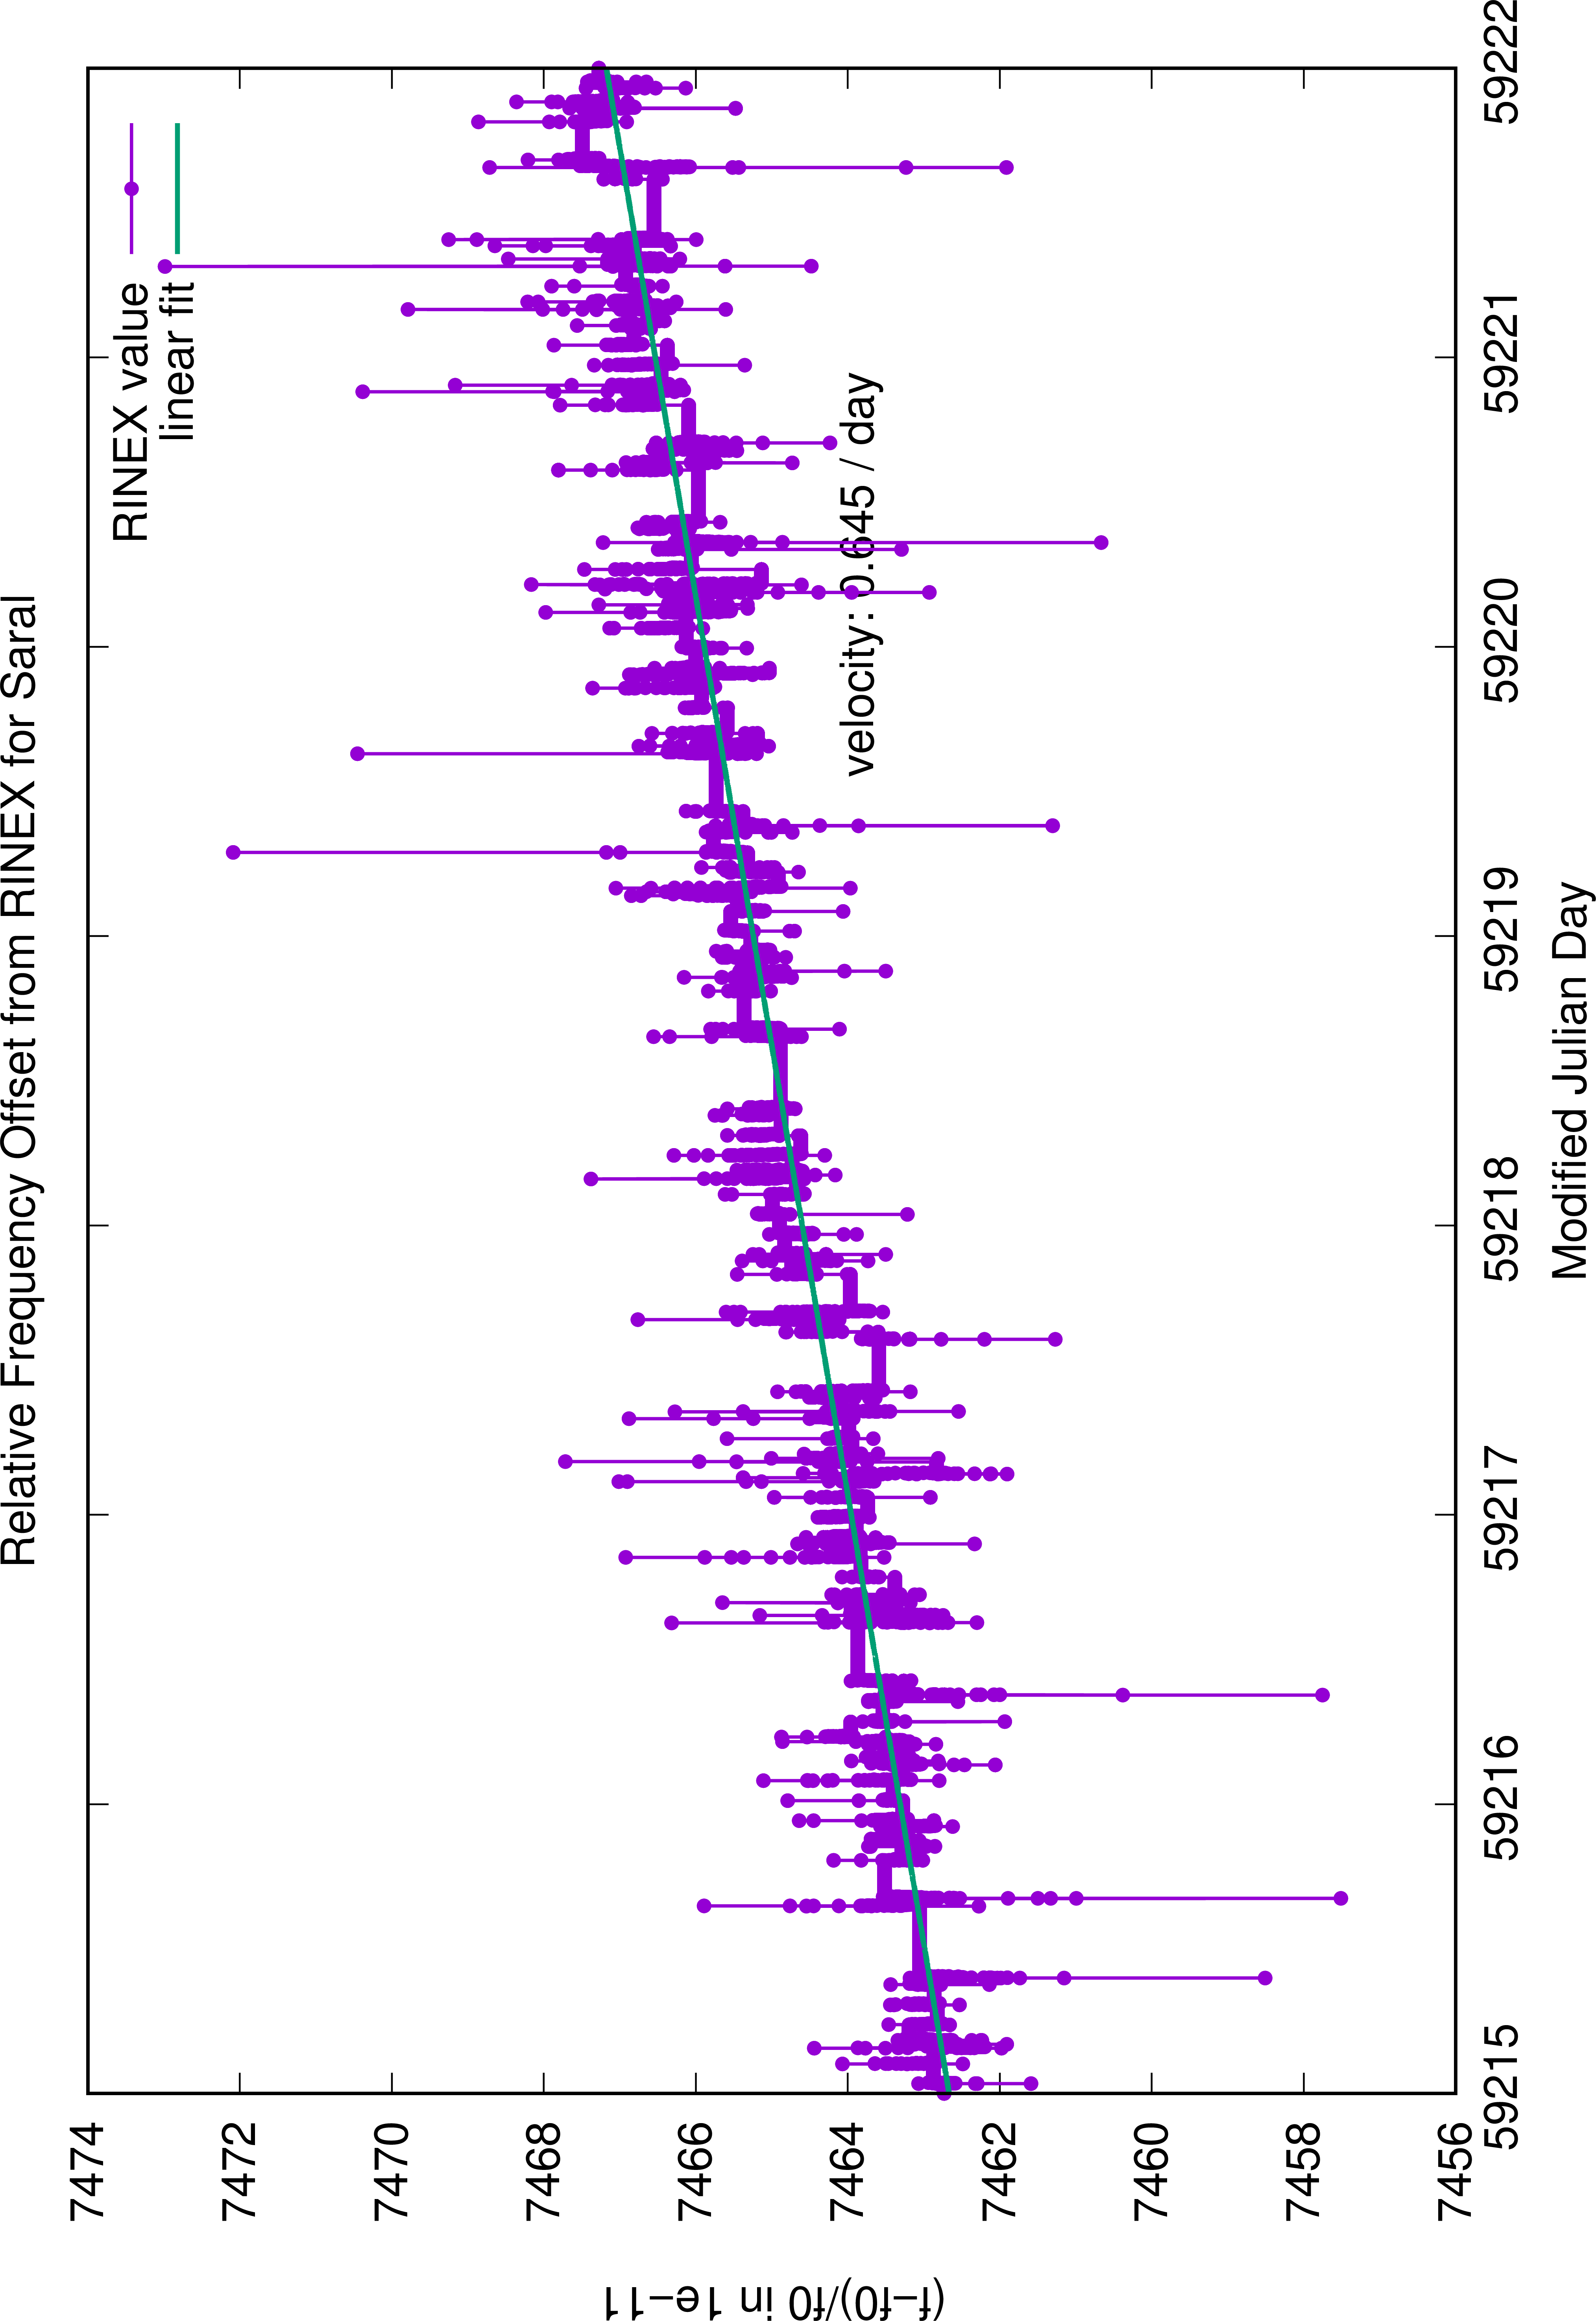
\includegraphics[scale=.3, angle=-90]{Saral-RinexRfo}
  \end{center}
\end{frame}

\begin{frame}\frametitle{Parameters}\framesubtitle{Delta Time \(\Delta\tau_r\)}
  \begin{equation*}
    \left.\begin{aligned}
        u_{measured} & = \frac{\color{red}c}{\color{red}f_{e_N}} 
          (\textcolor{red}{f_{e_N}} - 
            \textcolor{red}{f_{r_T}} -
            \frac{\color{red}N_{DOP}}{\Delta\tau_r}) + 
          \Delta u_{{REL}_C} + 
          \Delta u_{IONO}\\
        u_{theo} &= \frac{\rho_2 - \rho_1}{\Delta\tau_r} + 
          \Delta u_{TROPO} - 
          \frac{\textcolor{red}c(\frac{\textcolor{red}{N_{DOP}}}{
            \Delta\tau_r
          } + 
          \textcolor{red}{f_{r_T}})}{\textcolor{red}{f_{e_N}}} 
          \textcolor{blue}{\frac{\Delta f_e}{f_{e_N}}}
    \end{aligned}
\right\}
\end{equation*}

\(\Delta\tau_r = \tau_{r2} - \tau_{r1}\), where \(\tau_{r1}\) is the beginning of reception 
of the the 1\textsubscript{st} cycle by the receiver, and 
\(\tau_{r2}\) the end of reception of the N\textsubscript{th} cycle by the receiver, \underline{in the 
proper time scale of the receiver}, that is ...

\end{frame}

\begin{frame}\frametitle{Parameters}\framesubtitle{Satellite-Beacon distance \(\rho\)}
  \begin{equation*}
    \left.\begin{aligned}
        u_{measured} & = \frac{\color{red}c}{\color{red}f_{e_N}} 
          (\textcolor{red}{f_{e_N}} - 
            \textcolor{red}{f_{r_T}} -
            \frac{\color{red}N_{DOP}}{\textcolor{red}{\Delta\tau_r}}) + 
          \Delta u_{{REL}_C} + 
          \Delta u_{IONO}\\
        u_{theo} &= \frac{\tikz[baseline]{
          \node[fill=red!35, ellipse, anchor=base]
          {$\rho_2 - \rho_1$};
        }
        }{\textcolor{red}{\Delta\tau_r}} + 
          \Delta u_{TROPO} - 
          \frac{\textcolor{red}c(\frac{\textcolor{red}{N_{DOP}}}{
            \textcolor{red}{\Delta\tau_r}
          } + 
          \textcolor{red}{f_{r_T}})}{\textcolor{red}{f_{e_N}}} 
          \textcolor{blue}{\frac{\Delta f_e}{f_{e_N}}}
    \end{aligned}
\right\}
\end{equation*}


\end{frame}

%\begin{frame}\frametitle{Parameters}\framesubtitle{SV coordinates}
%    Extract satellite coordinates (or bettter yet state vector) from Sp3 files 
%    using some kind of interpolation.\\
%    \vspace{.2cm}
%    
%    At this point use polynomial interpolation using a (slightly modified) Neville's \citet{numrec3}
%    method.\\
%    \vspace{.2cm}
%    
%    Functions for reading/parsing Sp3 files are included in \href{https://github.com/xanthospap/sp3}{sp3}
%
%    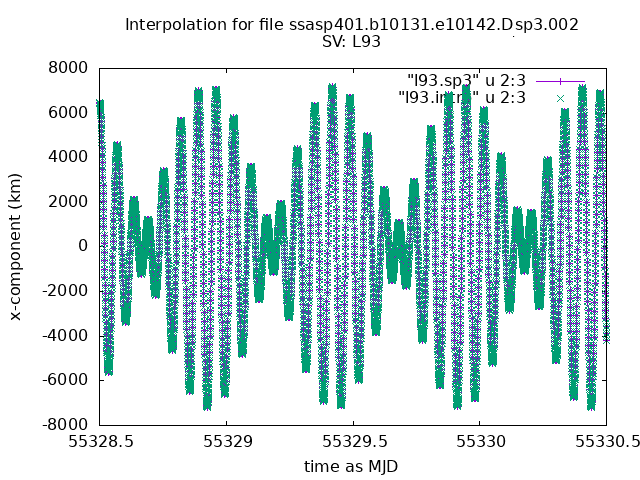
\includegraphics[scale=.4]{l93x}
%\end{frame}

\begin{frame}\frametitle{Parameters}\framesubtitle{Station/Beacon coordinates}
    Extract station coordinates in ITRF2014\\
    \vspace{.3cm}

    Implementation ready (for all stations included in the corresponding .psd files).\\
    \vspace{.3cm}

\end{frame}

\begin{frame}\frametitle{Parameters}\framesubtitle{Time tagging}
    Quite complicated in DORIS ....
    \vspace{.3cm}

    Synchronize to TAI\\
    \vspace{.3cm}

  \begin{itemize}
      \item Use RINEX data (clock offsets) \textcolor{red}{use this first}
      \item Model clock using own model
  \end{itemize}
    \vspace{.3cm}

\end{frame}

\begin{frame}\frametitle{Parameters}\framesubtitle{Antenna PCO/PCV}
    Corrections for phase centre offset/variations\\
    \vspace{.3cm}

  Implemented for all ground antenna types,
  \begin{itemize}
      \item Alcatel
      \item StarecB/StarecC
  \end{itemize}
  \vspace{.3cm}

  Not yet implemented for SV's
  \vspace{.3cm}

\end{frame}

\bibliography{doris}

\end{document}
